\chapter{PROJECT OVERVIEW}

%Replace \lipsum with text.
% You may have as many sections as you please. This is just for reference.



In this project we will present a Network Virtualisation solution using technique called Software Defined Network (SDN). We will start with the motivation behind the project and the problem statement subsequently.



\section{Motivation}

The motivation behind the project lies within the benefits that network virtualisation provides over traditional networking. The advantages of virtualisation has already been seen in the server and storage virtualisation. Some of the benefits are as follows:-

\begin{itemize}
    \item provides the centralised control over the network
    \item avails use of less money, time and effort on the hardware
    \item Technical skills requirement is lesser
    \item Application delivery time is reduced considerably
    \item Security is improved
    \item Reduction in recovery time in case of hardware failure
\end{itemize}

\section{Problem Statement}

After getting acquired with baadal networking stack, virtual network management in baadal and various virtual network management schemes, we came up with the following problem statement:-
\subsection{Understanding Baadal networking architecture}
In this part, we studied the baadal networking architecture so that we can see the applicability of the solution of the SDN to it.
\subsection{Introducing the SDN based control in Baadal using Floodlight}
As different SDN controllers are available for implementing SDN based solution, we studied various controllers like POX, OpenDayLight (ODL), FLoodLight etc. We experimented initially with POX, then ODL and finally moved to floodlight.
\subsection{Policy control design for the InterVLan communication}
In Baadal, VMs belonging to the different VLAN cannot communicate by default. But there can be a requirement of communication between two specific VMs belonging to different Vlan. So we designed a solution which enables intervlan communication between two specific VMs.

\subsection{Traffic Measurement among VMs and VM consolidation}
Under this, we measured the traffic between different VM using flows installed by the floodlight, and then consolidating VMs talking frequently on a single host.

\subsection{Observation and Comparison of Results}
After implementing the SDN based solution in baadal sandbox, we compared the performance of the intervlan networking with the default (Non SDN based) solution in terms of bandwidth.  

% You may add figures in the following manner.
% \begin{figure}[here]
% \begin{center}	
% 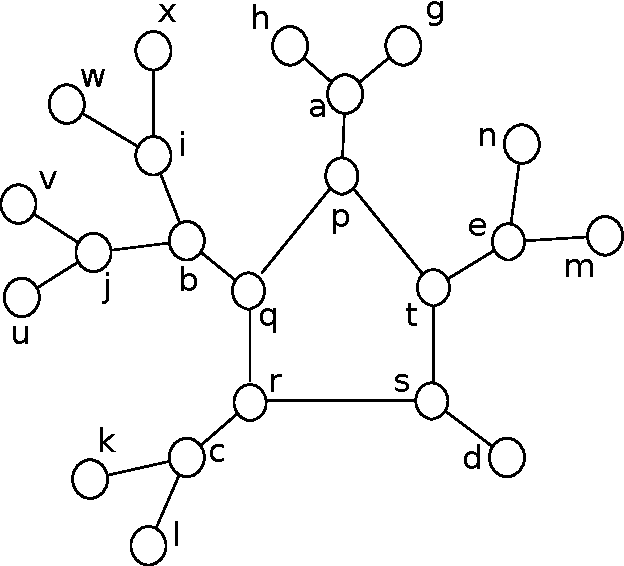
\includegraphics[scale=0.4]{pent} 
% \caption{Pentagon $pqrst$}
% \label{fig:pent}
% \end{center}
% \end{figure}



